\section{Results}
We evaluated the effect of imputation by drawing subsets of the BD2009 training set for the well-characterized allele HLA-A*02:01. Predictors were trained on a range of simulated training set sizes and tested on the remaining data (Figure ~\ref{fig:imputecomparison}). We find that imputation gives a modest improvement up to approximately 100 training samples. With more training data there is no benefit to imputation. The results are similar for the two other performance metrics (not shown).

% The figure doesn't show up in the preview but does show up if you export to pdf.
\begin{figure}[htb]
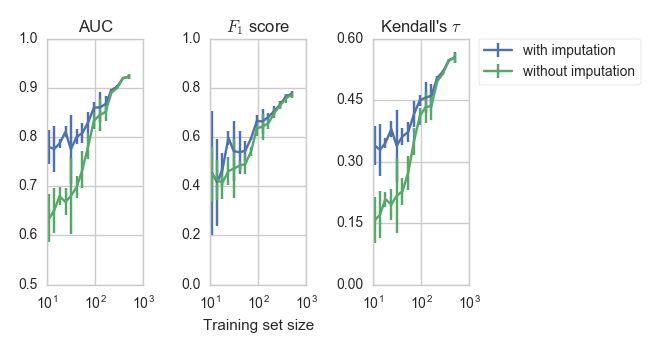
\includegraphics[scale=0.8]{figures/HLA-A0201-vs-nsamples-hidden-64-activation-tanh-impute-mice-epochs-250-embedding-32.png}
\caption{MHCflurry performance on down-sampled training data for HLA-A*02:01 (with and without imputation)}
\label{fig:imputecomparison} 
\end{figure}

We then compared the performance of MHCflurr against NetMHC, NetMHCpan, and SMM on the blind test data. The MHCflurry ensemble model contains 10 predictors initialized with different random weights. MHCflurry is competitive with both of these predictors.

\begin{table}[hb]
\centering
\begin{tabular}{llll}
\toprule
{} &               AUC &       $F_1$ score &  Kendall's $\tau$ \\
\midrule
MHCflurry (ensemble)        &  \textbf{0.93260} &           0.78459 &   \textbf{0.58686} \\
MHCflurry (single predictor)    &           0.93225 &           0.78106 &           0.58572 \\
NetMHC                          &           0.93234 &  \textbf{0.80722} &   \textbf{0.58633} \\
NetMHCpan                       &  \textbf{0.93264} &           0.79957 &           0.58138 \\
SMM-PMBEC                       &           0.92134 &           0.79026 &           0.56488 \\
\bottomrule
\end{tabular}

\caption{Performance on BLIND}
\label{tab:measurementweighted}
\end{table}

\section{Discussion}
Imputing training data shows promise in cross-validation as a way to improve performance on alleles with few observations, but only seems to help for very small training sizes ($\leq 200$). Unfortunately, only one allele in the BLIND dataset had fewer than 200 samples. Thus, additional work is required to assess the accuracy of MHCflurry and other predictors on alleles with very few training examples. Additionally, we need to further investigate the interaction between imputation parameters, the schedule according to which the weights of imputed samples are decayed, and stopping criteria for training individual allele-specific predictors. Nonetheless, even in its preliminary state, MHCflurry 

% These are generated in the 'paper plots' notebook; do not edit by hand.
